\documentclass[12pt]{report}
% \usepackage{minted}
\usepackage{xcolor}
\definecolor{light-gray}{rgb}{0.9,0.9,0.9}
% \usepackage{emptypage}
\usepackage[T1]{fontenc}
\usepackage{textcomp}
\usepackage[utf8]{inputenc}
% \usepackage[italian]{babel}
\usepackage{graphicx}
\graphicspath{ {Images/} }
\usepackage{caption}
\usepackage{subcaption}
\usepackage{enumerate}
\usepackage{array}
\usepackage{tabularx}
\usepackage{float}
\usepackage[a4paper,width=150mm,top=30mm,bottom=30mm,left=30mm,right=30mm,bindingoffset=6mm]{geometry}
\usepackage{fancyhdr}
\linespread{1.3}\selectfont

\usepackage{titlesec}
\titleformat{\chapter}{}{}{0em}{\bf\LARGE}

\usepackage{hyperref}
\hypersetup{
    colorlinks,
    citecolor=black,
    filecolor=black,
    linkcolor=black,
    urlcolor=black
}


\begin{document}
  %TODO: run a spellcheck
  %TODO: check id SafeStreets is well written in all files (i.e. missing final s)
  % TODO: Fill title page
  \begin{titlepage}
    \begin{figure}[t]
        \centering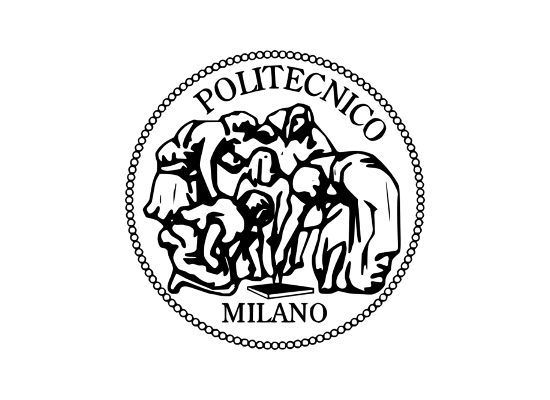
\includegraphics[width=0.5\textwidth]{Images/logo_polimi}
    \end{figure}
    \begin{center}
        \textsc{ \LARGE{Politecnico di Milano \\}}
      \textsc{ \LARGE{Dipartimento di Energia, Informazione e Bioingegneria\\ }}
      \textnormal{ \LARGE{Computer science and engineering \\ Software engineering 2\\}}
      \vspace{30mm}
      \fontsize{10mm}{7mm}\selectfont 
        \textup{SafeStreets - RASD}\\
    \end{center}
    
    \vspace{25mm}
    
    \begin{minipage}[t]{0.47\textwidth}
      \textnormal{\large{\bf Professor:\\}}
      {\large Prof. Elisabetta Di Nitto}
    \end{minipage}\hfill\begin{minipage}[t]{0.47\textwidth}\raggedleft
      \textnormal{\large{\bf Candidates:\\}}
      {\large Nicolò Albergoni - 939589\\}
      {\large Luca Loria - 944679}
    \end{minipage}
    
    \vspace{20mm}
    
    \centering{\large{Academic Year 2109/2020 \\ Milano - 10/11/2019 }}
    
  \end{titlepage}
  
  
  \tableofcontents
   
  \chapter{Introduction}
  \section{Purpose}
  The purpose of this Requirement Analysis and Specification Document (RASD)
is to provide a detailed description about SafeStreets.
In particular, this document is focused on important aspects that are
useful during the design of the software architecture like: scope, functional and
non-functional requirements, use cases and scenarios, constraints and assumption, UML diagrams, limitation and interfaces with other software.
Overall the document is a useful guide for the developers that will have to follow
and implement all the necessary requirements; nevertheless it is also a document
that can be given to potential customers to get them an idea of what the software
will be like.\newline
The software features have been identified in the following list of goals.

\subsection{Goals}
\begin{itemize}
  \item {[G1]}: Allow a person to become a registered User after submitting his credentials for the registration to the service
  \item {[G2]}: Allow the user to send a violation report consisting in a picture and some metadata
    \begin{itemize}
      \item {[G2.1]}: Allow the user to send along with the picture the plate number
    \end{itemize}
  \item {[G3]}: Allow the user to watch the history of his reports and their status
  \item {[G4]}: Allow the user to watch on a map areas and streets with an high frequency of violations
  \begin{itemize}
    \item {[G4.1]}: The user gets the latest violations near its current location 
    \item {[G4.2]}: The user gets the latest violations near the location that he specifies
  \end{itemize} 
  \item {[G.5]}: Allow the local system administrator of the police station to create accounts for the police technician by giving him an administrator account
  \item {[G.6]}: Allow the authorities to visualize the reports submitted by the users
  \item {[G.7]}: Allow the authorities to mine the data to make analisys and retrieve statistics
  \item {[G.8]}: If the municipality offers a service that provides data about accidents then the system must be able to cross this data with its own data in order to identify possible unsafe areas
  \begin{itemize}
    \item {[G.8.1]}: In this case the system must be able to suggest possible interventions
    \item {[G.8.2]}: The users must be able  watch this unsafe areas
    \item {[G.8.3]}: The authorities must be able to consult the crossed data
  \end{itemize} 
\end{itemize}


  \section{Scope}
  % TODO: check the scope
Here is a brief review of what has already been said into the RASD document about the SafeStreet scope and functionalities.
\newline
SafeStreets is a new service that aims, via the help of citizens, to improve the safety of the streets. Users will have the possibility to send reports of illegal behaviour related to street parking to authorities, just by opening the safe SafeStreets mobile application and take a picture of the violation. Moreover they can also consult the history of their reports and a map that will highlight the most dangerous streets nearby. SafeStreets also offers a way for the authorities to manage the reports and perform analysis on the data. A Web interface will be developed in order to address this purpose. In order to guarantee and efficient use of the application by authorities, the system interacts with an external plate recognition service that will extract the car plate number from the report image. In this way when authorities need to check on a report they immediately find the car plate number of the vehicle that committed the violation. SafeStreets also implements a functionality that performs the interaction with a municipality service that offers data regarding car accidents, if the particular municipality offers one. SafeStreets can cross this information with its owns, in order to get a better idea of the potentially unsafe areas and therefore suggest some possible interventions.
As for the performances, the service will have to be scalable,
fast and it must be able to cover a great number of users. While for the applications they must be lightweight and must run of most of the devices available on the market.

  \section{Definitions, acronyms and abbreviations}
  \subsection{Definitions}
\begin{itemize}
  \item \textit{Most Dangerous Streets}: Streets with the highest frequency of violation reports.
\end{itemize}

\subsection{Acronyms}
\begin{itemize}
  \item EU: European Union;
  \item CET: Central European Timezone;
  \item API: Application Programming Interface;
  \item HTTP: Hyper Text Transfer Protocol;
  \item GPS: Global Positioning System;
  \item GDPR: General Data Protection Regulation;
  \item REST: Representational State Transfer.
  \item URL: Uniform resource locator
  \item URI: Uniform resource indicator
  \item DB: Database
  \item DBMS: Database management system
  \item RDBMS: Relational database management system
  \item SQL: Structured query language
  \item NoSQL: Not only SQL
\end{itemize}

\subsection{Abbreviations}
\begin{itemize}
  \item {[Gn]}: n-th goal;
  \item {[Dn]}: n-th domain assumption;
  \item {[Rn]}: n-th functional requirements;
  \item MDS: Most Dangerous Street;
  \item LSA: Local System Administrator;
  \item PT: Police Technician.
\end{itemize}

  \section{Revision History}
  \begin{itemize}
    \item Version 1:
        \begin{itemize}
            \item 1.0: First release.
            \item 1.1: Minor fixes to sequence diagrams
        \end{itemize}
\end{itemize}

  \section{References}
  \begin{itemize}
    \item LateX Workshop extension for Visual Studio Code: \newline\href{https://github.com/James-Yu/LaTeX-Workshop/}{https://github.com/James-Yu/LaTeX-Workshop/}
    \item LateX compiler: \newline\href{https://www.latex-project.org/}{https://www.latex-project.org/}
    \item StarUML for UML diagrams:\newline\href{http://staruml.io/}{http://staruml.io/}
    \item DrawIO for some UML diagrams\newline\href{http://draw.io}{http://draw.io}
    \item MVC design pattern wikipedia: \newline\href{https://en.wikipedia.org/wiki/Model-view-controller}{https://en.wikipedia.org/wiki/Model-view-controller}
    \item Multitier architecture wikipedia: \newline\href{https://en.wikipedia.org/wiki/Multitier_architecture}{wikipedia}
    \item Relational database advantages: \newline\href{https://searchdatamanagement.techtarget.com/definition/relational-database}{https://searchdatamanagement.techtarget.com/definition/relational-database}
\end{itemize}
  \section{Document Structure}
  % TODO: check if this list is still right
\begin{enumerate}
  \item In the first part a general introduction of the Design Document is given. The purpose part exposes the substantial differences with the RASD document;
  \item The second section it's the core of the DD: it firstly provides an high level overview of the system followed by  a description of various aspects of the architecture from different points of view such as: component, deployment and runtime view. It is also present a general explanation of the architectural patterns and styles adopted in the development process. Most of the parts of this section are enriched with UML diagrams to ensure a better understanding of the concepts;
  \item This part specifies the user interface design of the mobile application and the web interface. Since the mockups of both applications were already provided in the RASD document, here some UX diagrams are proposed to better describe the navigation and functioning of the applications;
  \item Part four exposes the requirements traceability matrix which maps the requirements stated in the RASD document with the corresponding design component;
  \item Chapter five provides the proposals for the implementation, integration and testing plans. This plans are created by taking into account, for each functionality, the importance for the customer and the difficulty of implementation/testing;
  \item The last part states the hours of work division and the tools used to create  all the part of this DD document.
\end{enumerate}

  
  \chapter{Overall Description}
  \section{Product perspective}
  SafeStreets is a software that needs to be fast and reliable in order to allow the user to send a report immediately after he detects a violation. The goal is to design an architecture that can offer a good level of performance with respect to scalability and portability. The system is splitted into three separate applications: a mobile front-end application for the users, a Web application for the authorities and a back-end system that manages all the operations. More in details, the user application is a light-weight crossplatform mobile client; with this approach, the client side is relieved from the computation and the result is a fast application for the users. With this mobile application, users can perform the main functions related to them, such as: registration, login, send reports, consult the history of his reports and watch a map with the MDS. The application is connected to the backend service, which is the part of the architecture that handles all the main operations regarding the elaboration of data. In fact, the backend is the core of the architetcure: it manages the incoming requests and handles the interaction with the third party system for the plate recognition. This is fundamental because the authorities need to receive the plate number in order to immediately identify the right veichle. This operation is done by sending the picture taken by the user to an external service that finds the plate number in the image and sends it back to the system as a string. Moreover the backend provides an interface that interacts with the cloud-based database in which the data will be saved. Finally, it provides the functions to compute (on request) the MDS and other useful metrics. As an optional feature the backend can be configured to interact with the municipality service that offers data about car accidents. In this case, the backend compares the information sent with the data stored in the database. Therefore, it tries to identify the potentially unsafe areas and suggests possible interventions.\newline The Web application takes advantage of the interactions with the remote database offered by the backend to provide a simple interface for the authorities in order to let them consult the stored data: they can query all reports, filter them by some specific criterias and analyze the data to get the statistics that they desire.
\begin{figure}[H]
    \centering
    \includegraphics[width=1.0\textwidth]{UML_diagrams/Class}
    \caption{Class diagram}
    \label{fig:class_diagram}
\end{figure}
\begin{figure}[H]
    \centering
    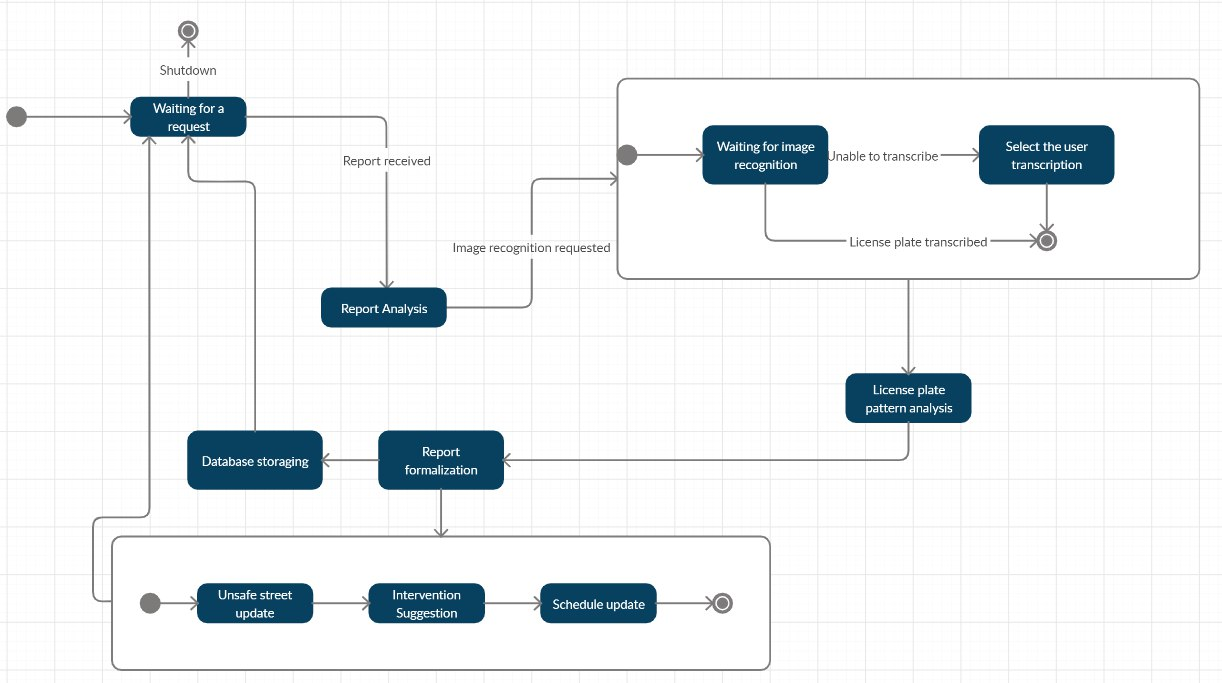
\includegraphics[width=1.0\textwidth]{UML_diagrams/State}
    \caption{Report state diagram}
    \label{fig:state}
\end{figure}
\newpage
  \section{Product Functions}
  \subsection{Send a report}
This is one of the most important function of the service. After the user has successfully registered/logged in to the application, he can choose to send a report of a violation to the officers. This is performed by taking a picture of the car that committed the violation. After the device took the picture the application asks the user to choose from a list of common violations the category that best describes the event (i.e. No parking zone, Double parking). When this information is provided the application gathers some other data in order to have a correct and useful report. In particular it gets: 
\begin{itemize}
  \item The data related to the user who wish to send the report (User ID);
  \item The local time and date gathered from the phone OS;
  \item The information about the street where the user took the picture (Obtained by the GPS coordinates of the user).
\end{itemize}

The user can also optionally add the car plate numbers and the name of the street in case, for example, the application misrecognized the street from the GPS coordinates. When all the necessary data are correctly gathered, the report is sent to the backend system that will handle the request. The user can then consult the history section of the application to monitor the status of its report.

\subsection{Receiving a report - Plate recognition}
The specification document states that the license plate needs to be extracted from the image in order to save it as a correct report. In order to extract the plate number from an image an external service is used. This choice was made because, for this kind of application, an established and robust, high accuracy recognition service will certainly work better than a recognition system that has to be built from scratch only for this kind of purpose. Therefore the backend system runs a task that listens for new reports and as soon as it receives a new one it immediately sends the image contained in the message to the plate recognition service. After the elaboration, the service returns the response of the recognition algorithm that should contain the text transcription of the plate. Note that if for some reason (i.e. bad picture) the plate recognition system can't recognize the plate, the backend system will instead use the plate number inserted by the user if provided; if not provided the violation won't be associated to any plate number. After this recognition step the backend system will interact with the database to create a record that contains the licence plate (if recognized/provided) and all the other information sent in the report. It is important to highlight the fact that the photo won't be discarded after the recognition as they can still be used for legal purposes.

\subsection{Information mining}
The system offers to both users and authorities the possibility to analyse the registered data although the level of visibility differs with respect to the utilizator. 
Users can only see the streets with the highest frequency of violations via the map present in the mobile application. Authorities instead have a wider access to data, that is to say they can access to all registered reports. Via the Web application they can also perform queries on the database (only selection queries) to mine the desired data and compute statistics and metrics for a deeper analysis. The role based approach has been designed in order to guarantee the privacy of car owners with respect to the users of the application. Therefore they will only be allowed to consult for the MDS.

\subsection{Scheduling technicians on violations}
The system offers to LSAs the possibility to manage the violation reports by scheduling them to one or more of their technicians.
Scheduled technicians will have the possibility to change the violation report status (from scheduled) to solved once they patrolled the street and confirmed/rejected the violation.

\subsection{Crossing data with the municipality}
The backend system offers the possibility to interact with an external service, offered by the municipality, that provides data regarding car accidents happened in the municipality area. SafeStreets can define the potential unsafe areas of the municipality by merging car accidents data and violation reports stored by the application. The system can then suggest to the local system administrator possible interventions in order to improve the safety of this areas. It is important to note that the data offered by this service need to be structured in a standard way recognizable by the backend system, otherwise the information crossing will not provide any results.

  \section{User Characteristics}
  \subsection{Actors}

\begin{itemize}
    \item \textit{Visitor}: a person without a SafeStreet account. Visitors can only have access to the homepage and the registration form of the mobile application;
    \item \textit{User/ Mobile user}: a person correctly registered to the SafeStreet account service. Users/Mobile users can perform any of the actions made available by the SafeStreet mobile application; 
    \item \textit{Recognized authority}: a recognized authority (Police station/ municipality) which submitted to SafeStreet and can interact with it through its web application interface;
    \item \textit{Local system administrator/Police corporal}: a person which belongs to a recognized authority, in charge of dealing police technician accounts and scheduling patrols;
    \item \textit{Police technician}: a policeman encharged of dealing with the violations report. He/She patrols the unsafe areas and gives fines to the reported cars in case of violations;
    \item \textit{Third party recognition service}: an image recognition service which allows SafeStreet to extract car plates from the violation report's images.
\end{itemize}


  \section{Assumptions and dependencies}
  As far as the specification document is concerned, it is necessary to specify some details and to state clearly a few ambiguous points. In order to better clarify those situations the following assumptions are intoduced.
\subsection{Text Assumptions}
\begin{itemize}
    \item \textbf{Violation report}
        \begin{itemize}
            \item The information sent by user in the violation report includes: the license plate image and an optional textual transcription, its position coordinates (extracted automatically from the smartphone GPS) and the violation metadata;
            \item The suitable metadata descripted in the specification document is intended as a choice of the law infringment and a textual description of the event;
            \item Given the coordinates of the violation, the system is able to retrieve the address from which the report was sent;
            \item Every time a report is received, the system will ask the image recognition service for the license plate textual transcription.
            \item A license plate textual transcription is considered correct if it fits into one of the common standard of the EU states. In case of wrong textual transcription of the license plate from the image recognition service:
            \begin{itemize}
                \item The textual transcription provided by the user is taken into account. After a previous check, the provided license plate will be considered as correct.
                \item If the user has not sent a textual transcription, the violation is not associated to any license plate number;
            \end{itemize} 
        \end{itemize}
    \item \textbf{Mining information} 
        \begin{itemize}
            \item End users are allowed to mine information about the violation reports that they sent. Also, they can have access only to the (map visualization or list) streets with the highest frequency of violation reports (called "most dangerous" streets (MDS) from now on);
            \item Authorities can mine information concerning all the stored information in the SafeStreet system, such as MDS or the list of cars with an high number of violation reports.
        \end{itemize}
    \item \textbf{Suggested intervention}
        \begin{itemize}
            \item Only authorities are allowed to have access to the suggested intervention on unsafe areas identified by the system.
        \end{itemize}
    \end{itemize}
\subsection{Domain assumptions}
\begin{itemize}
    \item {[D1]}  A picture taken with a smartphone is performed with a quality sufficient for the image recognition service to transcribe it;
    \item {[D2]}  The reported picture contains only the license plate of the car that committed the violation and not others;
    \item {[D3]}  The GPS information collected from the smartphone of a user has an accuracy of less than 5 meters;
    \item {[D4]} The timestamp collected from the smartphone is synchronized with the CET standard;
    \item {[D5]} The users can only report violations occured in Europe;
    \item {[D6]} Reports are only sent through a secure connection channel;
    \item {[D7]} The users reports all the violation that they detect;
    \item {[D8]} The users send report containing correct information about the detected violation;
    \item {[D9]} The municipality system stores correctly all the information concerning car accidents;
    \item {[D10]} The municipality legacy system allows SafeStreet to retrieve information about the car accident among a certain area;
    \item {[D11]} The image recognition service is able to detect and transcribe license plates;
\end{itemize}



  
  \chapter{Specific requirements}
  \section{External interface requirements}
  \subsection{User Interfaces}
This section shows a mockup version of the main functionalities of the mobile application and the web application of the final version of SafeStreets.
\begin{itemize}
    \item Mobile application:
            \begin{figure}[H]
                \centering
                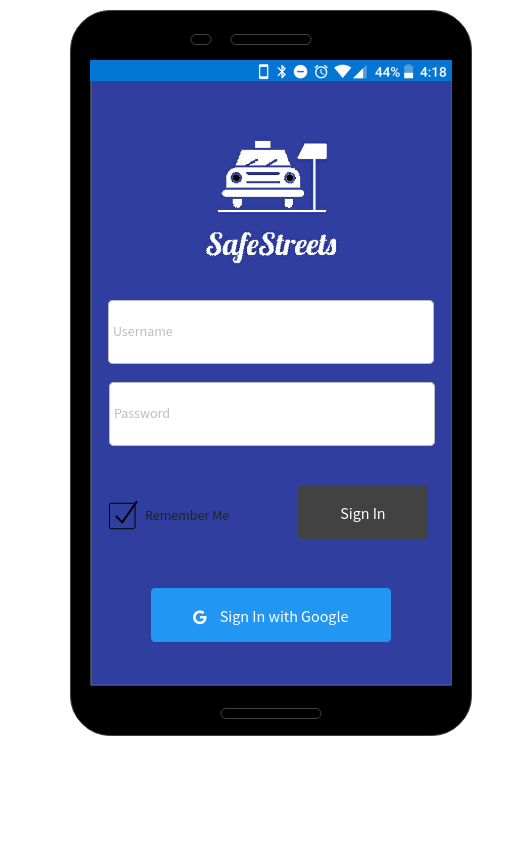
\includegraphics[width=0.45\textwidth]{login_app}
                \caption{LogIn interface}
                \label{fig:login_app}
            \end{figure}
            The Figure \ref{fig:login_app} represents the login form of the SafeStreets
            mobile application. The user can login through his username
            and password, or his Google account.
            \begin{figure}[H]
                \centering
                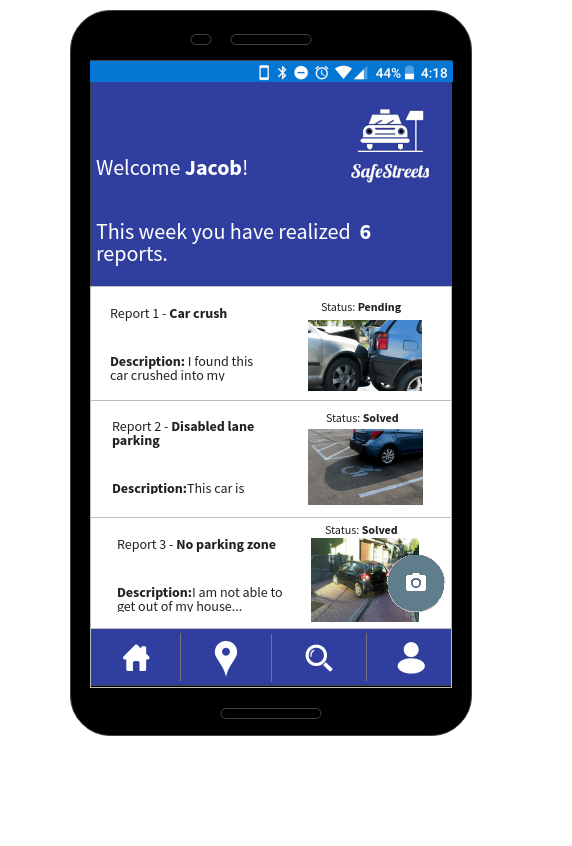
\includegraphics[width=0.45\textwidth]{home_app}
                \caption{Homepage}
                \label{fig:home_app}
            \end{figure}
            The figure \ref{fig:home_app} represents the homepage of the SafeStreets
            mobile application. The user is allowed to look at the list
            of the violation reports that he published, publish a new one
            through the floating button or visit other sections of the app.
            \begin{figure}[H]
                \centering
                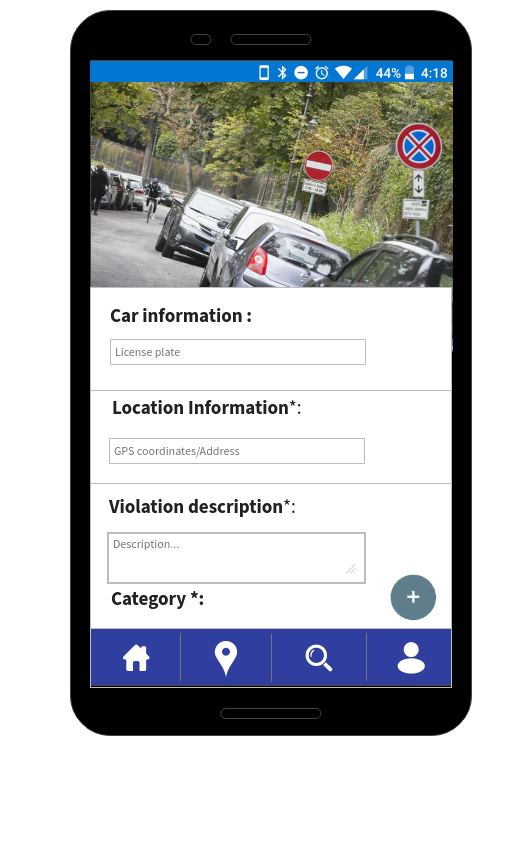
\includegraphics[width=0.45\textwidth]{violations_app}
                \caption{Violation report publishing page}
                \label{fig:violations_app}
            \end{figure}
            The figure \ref{fig:violations_app} represents the violations report
            publishing page of the SafeStreets mobile application. 
            The user is allowed take a picture of the violation clicking on the camera
            button and fill in the form to realize the violation report.
            \begin{figure}[H]
                \centering
                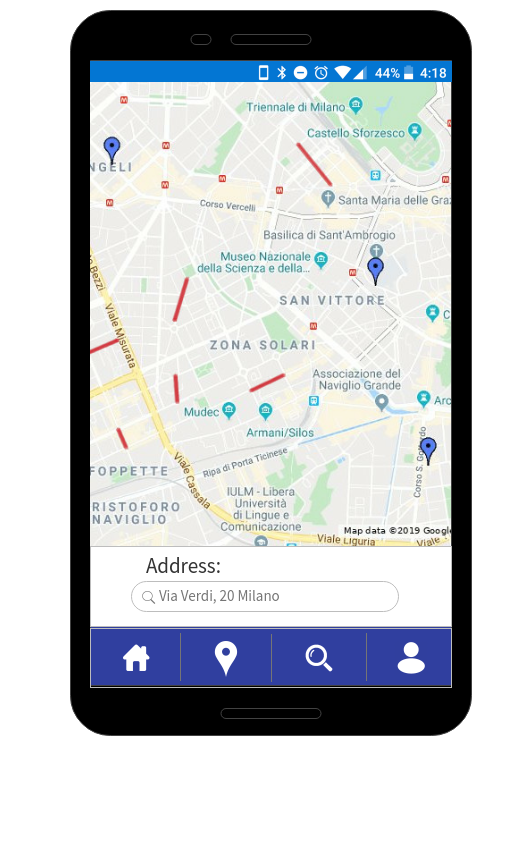
\includegraphics[width=0.45\textwidth]{maps_app}
                \caption{Map search page}
                \label{fig:maps_app}
            \end{figure}
            The figure \ref{fig:maps_app} represents the map page of the SafeStreets mobile application. 
            The user is allowed to look at the MDS highlighted in red on the map. It is also
            possible to search for a specific address through the search bar.
            \newpage
    \item  Web application;
    \begin{figure}[H]
        \centering
        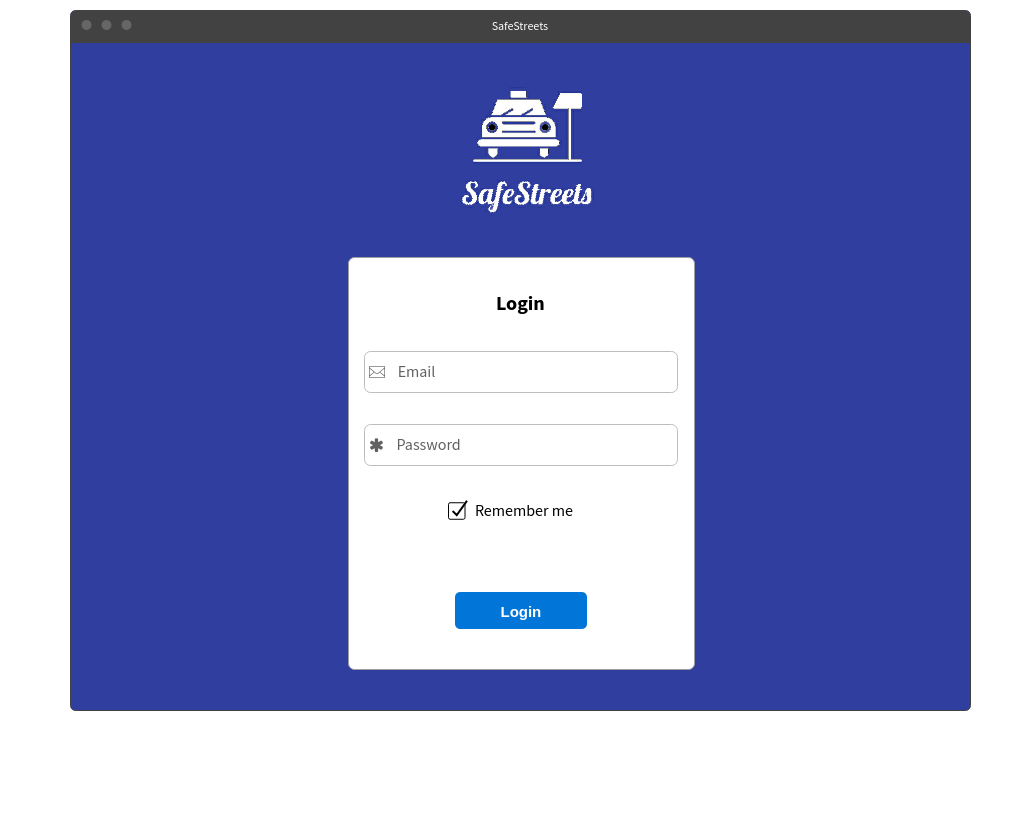
\includegraphics[width=0.75\textwidth]{login_web}
        \caption{LogIn interface}
        \label{fig:login_web}
    \end{figure}
    The Figure \ref{fig:login_web} represents the login form of the SafeStreets
    web application. The officer can login through his username
    and password.
    \begin{figure}[H]
        \centering
        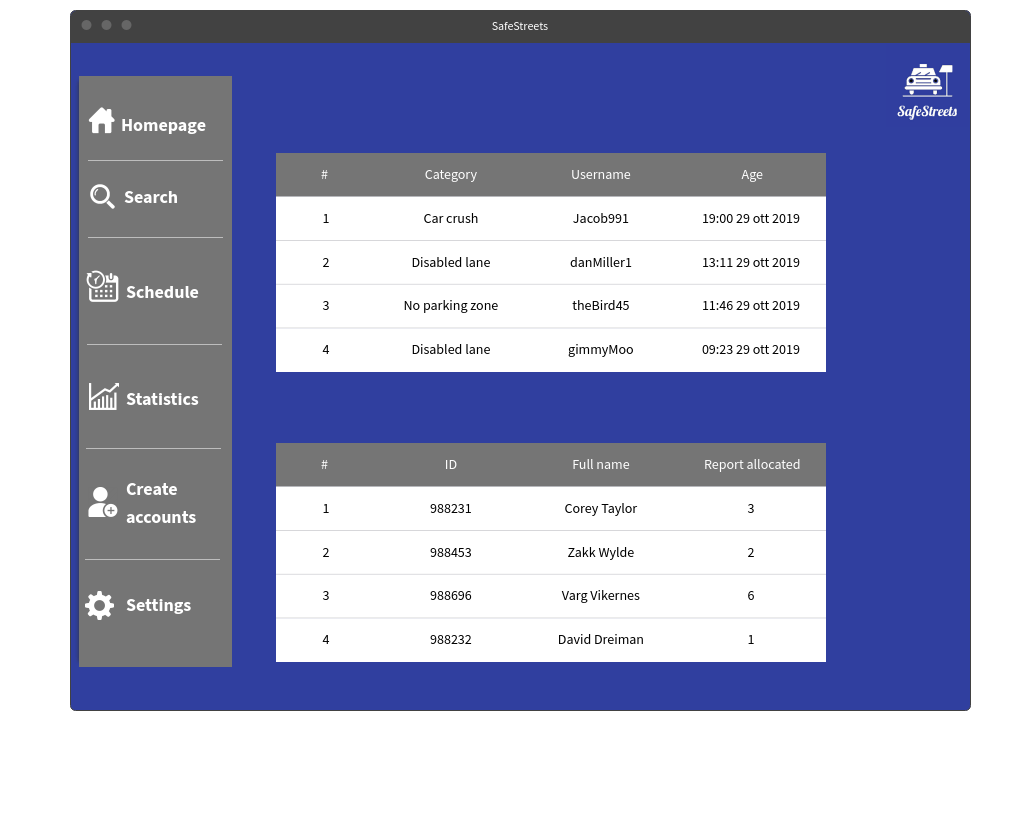
\includegraphics[width=0.75\textwidth]{home_web}
        \caption{Homepage}
        \label{fig:home_web}
    \end{figure}
    The figure \ref{fig:home_web} represents the homepage of the SafeStreets
    web application. The local system administrator is able to look at the list
    of recent violations, the list of the registered police technicians or to visit
    other pages by the side menu.
    \begin{figure}[H]
        \centering
        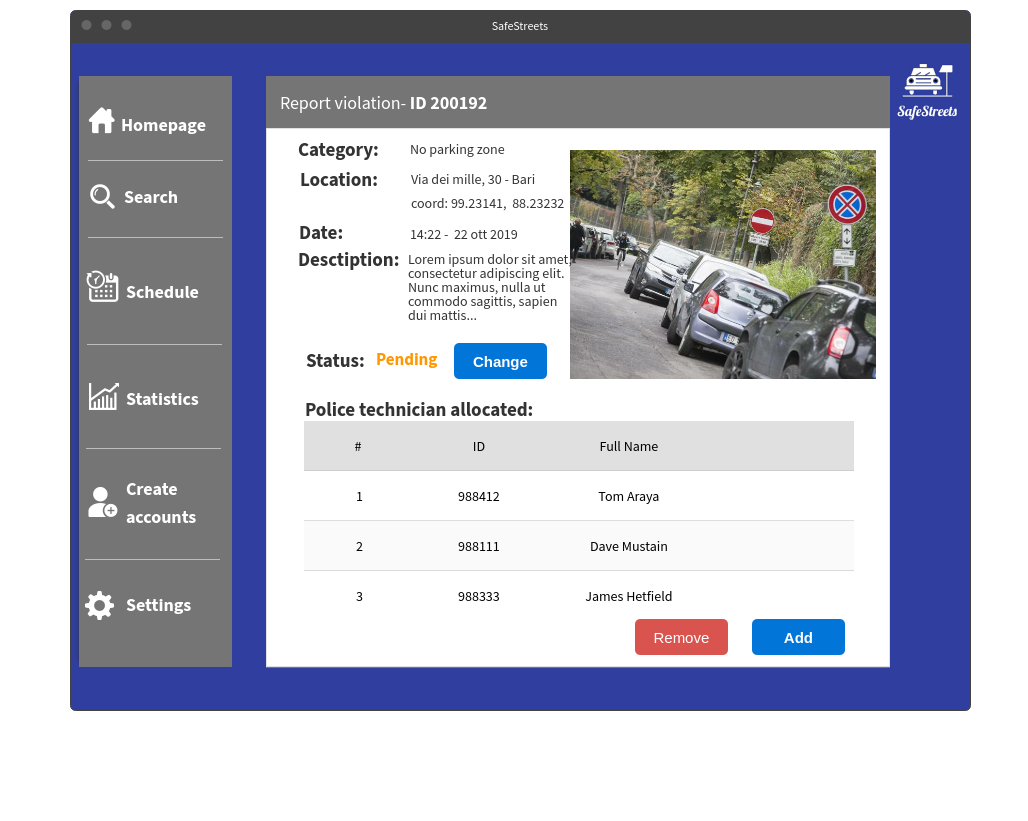
\includegraphics[width=0.75\textwidth]{report_web}
        \caption{Specific violation report page}
        \label{fig:report_web}
    \end{figure}
    The figure \ref{fig:report_web} represents the specific violations report
    page of the SafeStreets web application. 
    Both the LSA and the PT are able to look at the full violation report and they can change the report status from Pending to Closed (or viceversa). However, the LSA only can allocate/deallocate police technicians from this specific report.
    \begin{figure}[H]
        \centering
        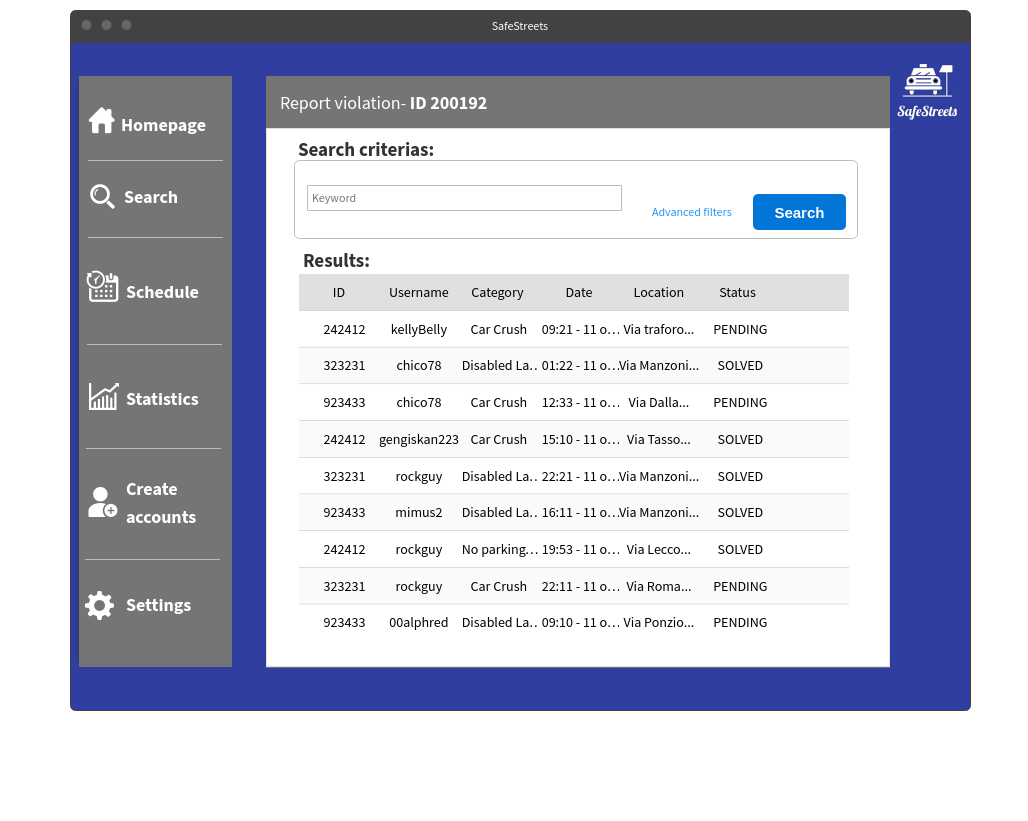
\includegraphics[width=0.7\textwidth]{mine_web}
        \caption{Report mining page}
        \label{fig:mine_web}
    \end{figure}
    The figure \ref{fig:mine_web} represents the report search page of the SafeStreets web application. 
    The local system administrator is able to search for a set of violation applying a keyword filtering
    and some advanced filters, such as date range or location.
\end{itemize}

\subsection{Hardware Interfaces}
SafeStreets do not require any specific hardware device, 
thus there are no hardware interfaces to other existing systems.
\subsection{Software Interfaces}
SafeStreets is a standalone service and does not share any API to 
external systems. However, the system requires the interaction with the Image recognition service and with the municipality's legacy system to perform its tasks. Also, a map service is required in order to show the MDS positions on the mobile application.\newline
The software requires a standard format in order to retrieve car accident.
data from the municipality's system. Such standard will be specified more in details in the DD.
\subsection{Communication Interfaces}
External services are not allowed to interact actively with SafeStreets, therefore the system does not offer any communication interface to external systems.

  \section{Functional Requirements}
  \subsection{Scenarios}
\subsubsection{Scenario 1}
John is a very sportsman person who likes to ride his bicycle a lot. Therefore, every Sunday afternoon he decides to go for a ride along the bicycle lane near his house. After some time he sees a car parked on the bike lane that limits the passage of bicycles. Thus, John decides to open up the SafeStreets application on his smartphone and takes a picture of the car. After that he selects the "No parking zone" as a violation category and adds the car plate number to the report in order to make sure that it will get correctly processed by the officers. 

\subsubsection{Scenario 2}
Albert's son, Freddy, has recently been operated to his leg. Thus, the municipality released him a pass which allows Albert to park in places reserved for people with disabilities. During the week, Albert has to take Freddy to the doctor for some checks. Sometimes, he manages to find a free parking spot in front of the hospital reserved for people with disabilities, but other times the place happens to be occupied by another car without a disabilities' pass. When this happens he needs to find another parking spot more distant from the hospital and therefore he his forced to make his son walk to the healthcare centre. This can be dangerous as he has just been operated. After some weeks in this condition, Albert decides to use the SafeStreets service in order to prove if the service can be really useful: he sends a report every time he finds himself in this kind of situation. After a certain period, he notices that the parking spots are either free or regularly occupied. In order to prove the functioning of the app, Albert checks his report history and finds out that all of his requests have been solved by the police.

\subsubsection{Scenario 3}
Every morning Kevin wakes up to go to work. Around 7 o'clock he leaves home to get to the parking spot where he parked his car the day before. Once he arrives at his car location, he notices that the car parked behind his' has crushed into his rear bumper leaving a noticeable dent. He does not have time to call the police because he is in a hurry for an important meeting at work, thus he decides to immediately send a crush report by taking a picture of the unpleasant event. After that, he rapidly gets on his car in order to arrive in time at work. Once he finishes his shift, he opens up the SafeStreets app to check the status of his report. Fortunately, he finds out that his request has been taken into account by a local police officer.

\subsubsection{Scenario 4}
Marco has been invited to Luigi's graduation party organized to celebrate his master degree in Computer Science and Engineering obtained at Politecnico di Milano. Marco lives in a small city with very limited public transportation solutions. In order to get to Milan, he decides to go with his car to the event. Once he is almost close to the designated place, he starts to looking for a parking spot. Soon later, he remembers that Luigi told him to download the SafeStreets app in order to check where the most unsafe streets in the area could be. He stops the car and opens the mobile application. Then, he navigates to the map section and finds on the map the location where the party is held. The application highlights the most dangerous streets near this location so that Marco can avoid parking his car there.

\subsubsection{Scenario 5}
Leon is a newly hired police technician at the Berlin police department. For his first days of work the corporal assigned  him some routine work, mainly focused on patrols and giving fines. In order to check where he needs to patrol, he logs into the SafeStreets Web application from his computer with his credentials. Once logged in, He consults the scheduled violation reports submitted by the police corporate, in order to find out their locations. 

\subsubsection{Scenario 6}
Daniele is the local system administrator of the Genova police department and he is responsible of dispatching patrols. He decides that he wants to schedule the officers in a more intelligent way. In order to do that, he consults the SafeStreets report database by logging in the web application. He would like to send the more experienced officers to areas in which there is a high number of violations categorized as "crash violations" whereas he would assign regular officers to other streets with an high frequency of violation of any category. In order to find out those streets, he filters the reported violations by the web application;immediately after, the interface displays the desired results. Now he is able to schedule the patrols as he wants. Daniele would also like to communicate which are the 10 cars that committed the highest number of violations in the city to all the officers. To do that he filters once again by the SafeStreets web application searching for the 10 car plates with the highest rate of violations.

% TODO: check if this is good enough
\subsubsection{Scenario 7}
Robert is a civil councillor encharged of the street's safety of the city. He would like to find out which are the possible interventions that can be performed on the city streets in order to provide a safer circulation. Robert has limited budget  and he wants to perform only the paramount interventions: he asks to a friend that works in the police department of the city to retrieve some suggestions using the newly purchased SafeStreets system. Robert knows that the SafeStreets system crosses the data offered by the municipality about car accidents with its own information about violations happened in the city. The system finds out that there is a relation between car accidents and unsafe parking in zones near biking lanes.Thus,in order to limit the number of incidents/violations, the system suggests to build barriers that divide the bike lane from the street. Robert likes the idea and start to work on a plan that he will propose to his manager.


\subsection{Use cases} \label{use_cases}
% \begin{tabular}{|p{3.7cm}|p{11cm}|}
%   \hline
%   Name & Sign Up\\
%   \hline
%   Actors & Visitor\\
%   \hline
%   Entry Condition & The visitor has opened the application on his device\\
%   \hline
%   Event flow & \begin{enumerate}
%                   \item The Visitor chooses the Sign Up option;
%                   \item The Visitor fills the mandatory fields regarding his personal data (i.e. email, password);
%                   \item The Visitor fills the optional fields (i.e. Name,Surname, age)
%                   \item The Visitor confirms the registration;
%                   \item The system saves the information and creates the User account.
%               \end{enumerate}\\
%   \hline
%   Exit condition & The User is registered.\\
%   \hline
%   Exception & \begin{enumerate}
%                 \item The user was already registered. In this case the application warns the user that there is another account associated to the specified email;
%                 \item The user does not fills all the mandatory fields. In that case the application warns the user by highlighting the empty fields.
%               \end{enumerate}\\
%   \hline
%   \end{tabular}

\newcolumntype{b}{X}
\newcolumntype{s}{>{\hsize=.5\hsize}X}

  \begin{tabularx}{\textwidth}{|s|b|}
    \hline
    Name & Sign Up\\
    \hline
    Actors & Visitor\\
    \hline
    Entry Condition & The visitor has opened the application on his device\\
    \hline
    Event flow & \begin{enumerate}
                    \item The Visitor chooses the Sign Up option;
                    \item The Visitor fills the mandatory fields regarding his personal data (i.e. email, password);
                    \item The Visitor fills the optional fields (i.e. Name,Surname, age)
                    \item The Visitor confirms the registration;
                    \item The system saves the information and creates the User account.
                \end{enumerate}\\
    \hline
    Exit condition & The User is registered.\\
    \hline
    Exception & \begin{enumerate}
                  \item The user was already registered. In this case the application warns the user that there is another account associated to the specified email;
                  \item The user does not fills all the mandatory fields. In that case the application warns the user by highlighting the empty fields.
                \end{enumerate}\\
    \hline
  \end{tabularx}
  



\subsection{Requirements}
\begin{itemize}
  \item \textbf{{[G1]}: Allow the user to send a violation report consisting in a picture and some metadata;}
    \begin{itemize}
      \item {[R1]}: The mobile application must be able to gather all the required data such as: location, date and time from the user's device;
      \item {[R2]}: The mobile application has to allow the user to choose between different categories of violations;
      \item {[R3]}: The mobile application has to allow the user to optionally add information about the event and the car plate number;
      \item {[R4]}: The mobile application has to allow the user to retake the picture if desired;
      \item {[R5]}: The mobile application must be able to interact with the backend system to send/retrieve information;
      \item {[R6]}: The backend system must be able to send the violation image to the plate recognition service in order to retrieve the car plate number from the image;
      \item {[R7]}: Once the car plate number has been retrieved the system must save the report information in the database;
      \item {[D1]}: A picture taken with a smartphone is performed with a quality sufficient for the image recognition service to transcribe it;
      \item {[D2]}: The reported picture contains only the license plate of the car that committed the violation and not others;
      \item {[D3]}: The GPS information collected from the smartphone of a user has an accuracy of less than 5 meters;
      \item {[D4]}: The timestamp collected from the smartphone is synchronized with the CET standard;
      \item {[D5]}: The users can only report violations occurred in Europe;
      \item {[D6]}: Reports are only sent through a secure connection channel;
      \item {[D7]}: The users reports all the violation that they detect;
      \item {[D8]}: The users send report containing correct information about the detected violation.
    \end{itemize}
  \item \textbf{{[G2]}: Allow the user to watch the history of his reports and their status;}
    \begin{itemize}
      \item {[R5]}: The mobile application must be able to interact with the backend system to send/retrieve information;
      \item {[R8]}: The backend system must retrieve the latest reports submitted by the user from the database. Once the data are gathered, the backend system must send them to the mobile application that will display them;
      \item {[R9]}: The user must be able to consult the status associated with each report;
      \item {[D6]}: Reports are only sent through a secure connection channel;
    \end{itemize}
  \item \textbf{{[G3]}: Allow the user to watch on map areas and streets with an high frequency of violations;}
    \begin{itemize}
      \item {[R5]}: The mobile application must be able to interact with the backend system to send/retrieve information;
      \item {[R10]}: The application has to allow the user to insert an address near which to search the MDS. If no address is provided the application will instead search the MDS near the current position of the user (collected from the GPS);
      \item {[R11]}: The backend system must calculate the MDS close to the given location;
      \item {[R12]}: The mobile application must enlighten on the map the MDS;
    \end{itemize}
  \item \textbf{{[G.4]}: Allow the local system administrator of the police station to create accounts for the police technicians;}
    \begin{itemize}
      \item 
    \end{itemize}
\end{itemize}


\newpage
\subsection{Sequence diagrams}
\begin{figure}[H]
  \centering
  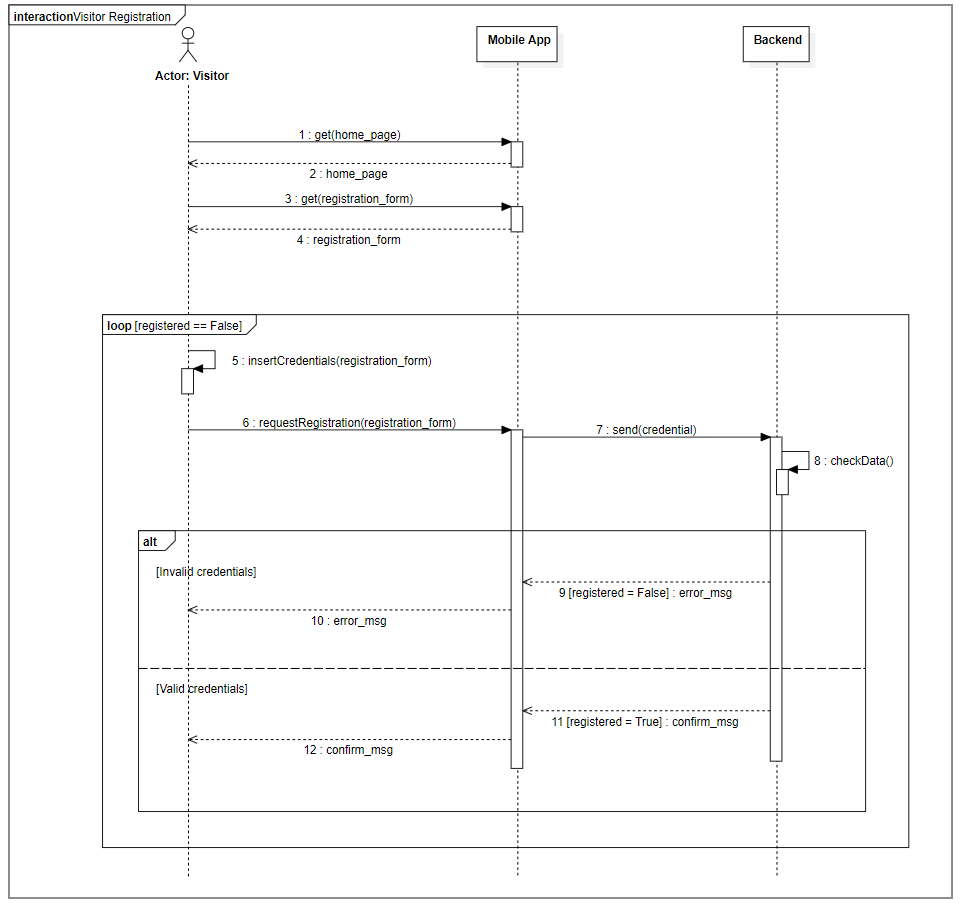
\includegraphics[width=\textwidth]{UML_diagrams/Sequence_Digrams/visitor_registration_sd.png}
  \caption{Visitor registration sequence diagram}
  \label{fig:visitor_signup_sd}
\end{figure}

\begin{figure}[H]
  \centering
  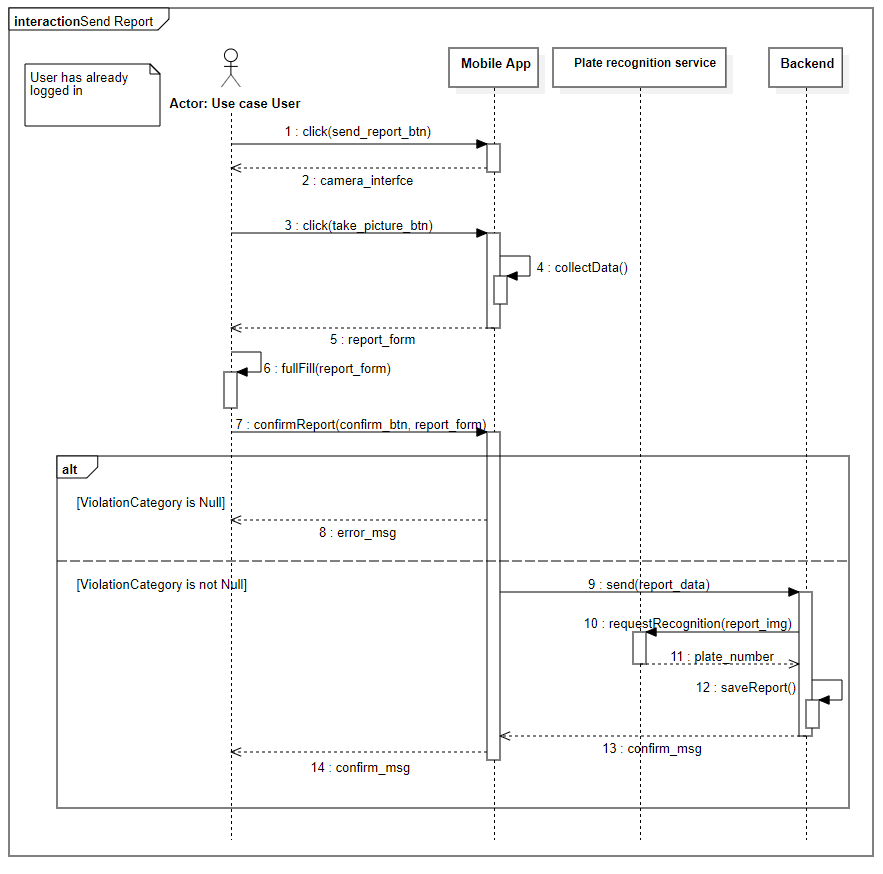
\includegraphics[width=\textwidth]{UML_diagrams/Sequence_Digrams/send_report_sd.png}
  \caption{Send report sequence diagram}
  \label{fig:send_report_sd}
\end{figure}

\begin{figure}[H]
  \centering
  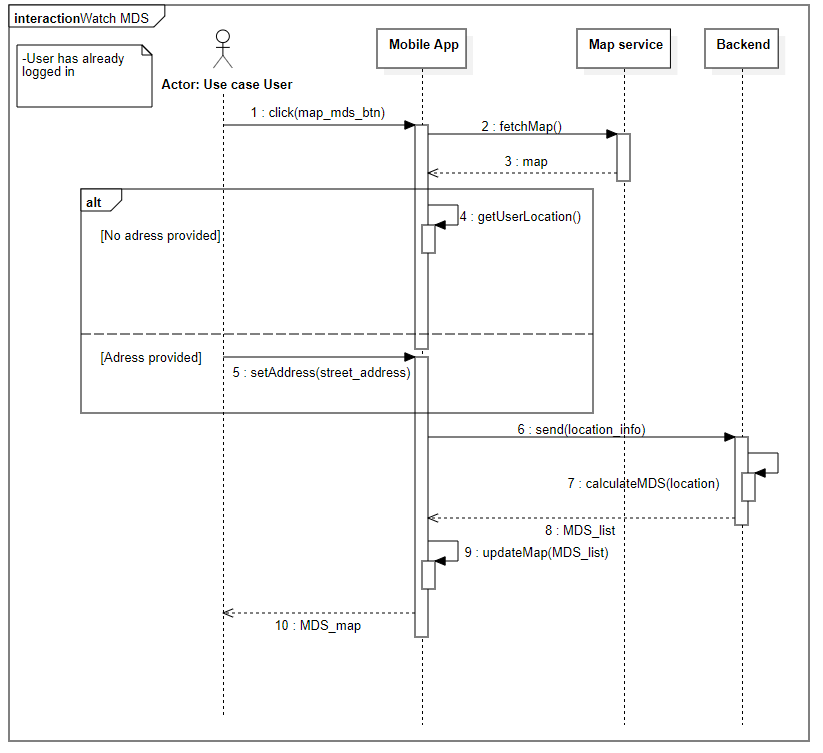
\includegraphics[width=\textwidth]{UML_diagrams/Sequence_Digrams/watch_mds_sd.png}
  \caption{Watch MDS sequence diagram}
  \label{fig:watch_mds_sd}
\end{figure}

\begin{figure}[H]
  \centering
  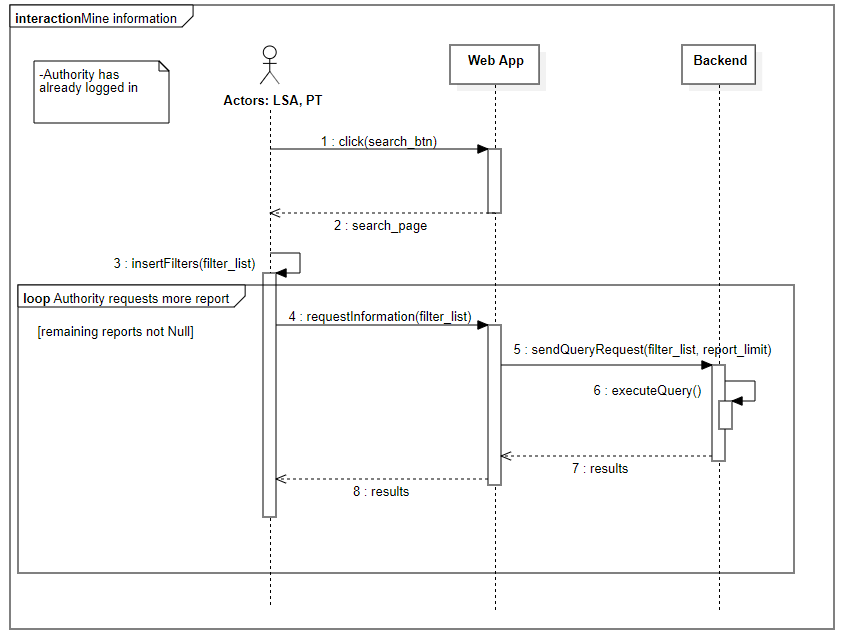
\includegraphics[width=\textwidth]{UML_diagrams/Sequence_Digrams/mine_information_sd.png}
  \caption{Mine information sequence diagram}
  \label{fig:mine_information_sd}
\end{figure}

\begin{figure}[H]
  \centering
  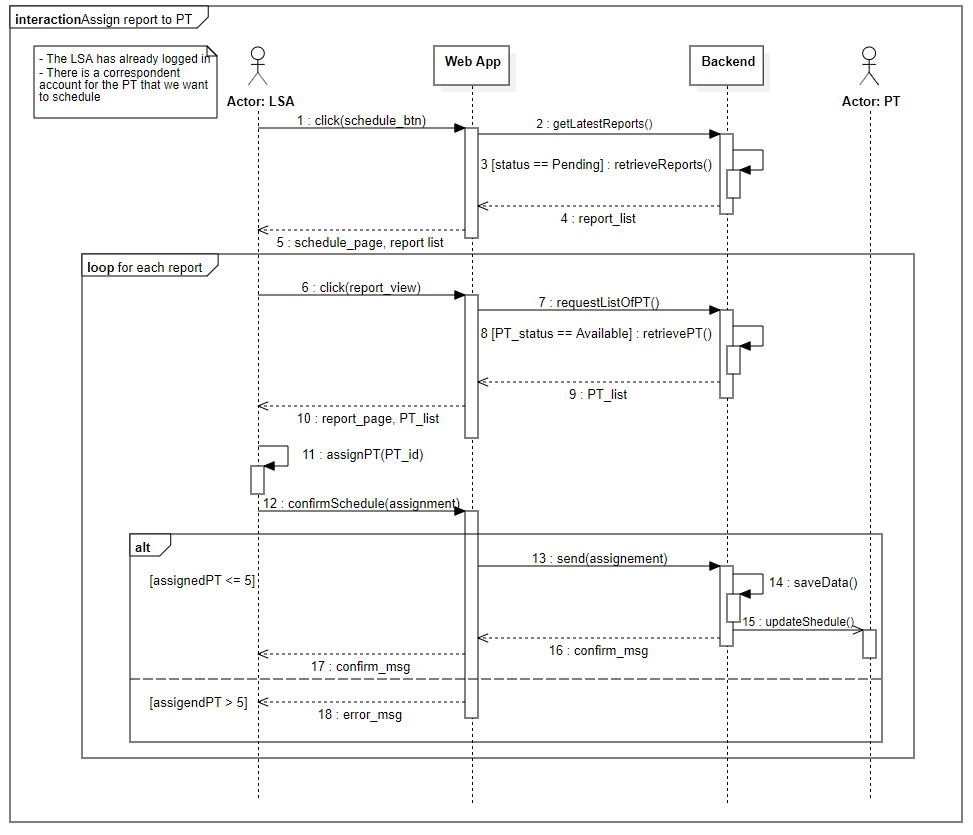
\includegraphics[width=\textwidth]{UML_diagrams/Sequence_Digrams/assign_PT_sd.png}
  \caption{Assign report to PT sequence diagram}
  \label{fig:assign_PT_sd}
\end{figure}

\begin{figure}[H]
  \centering
  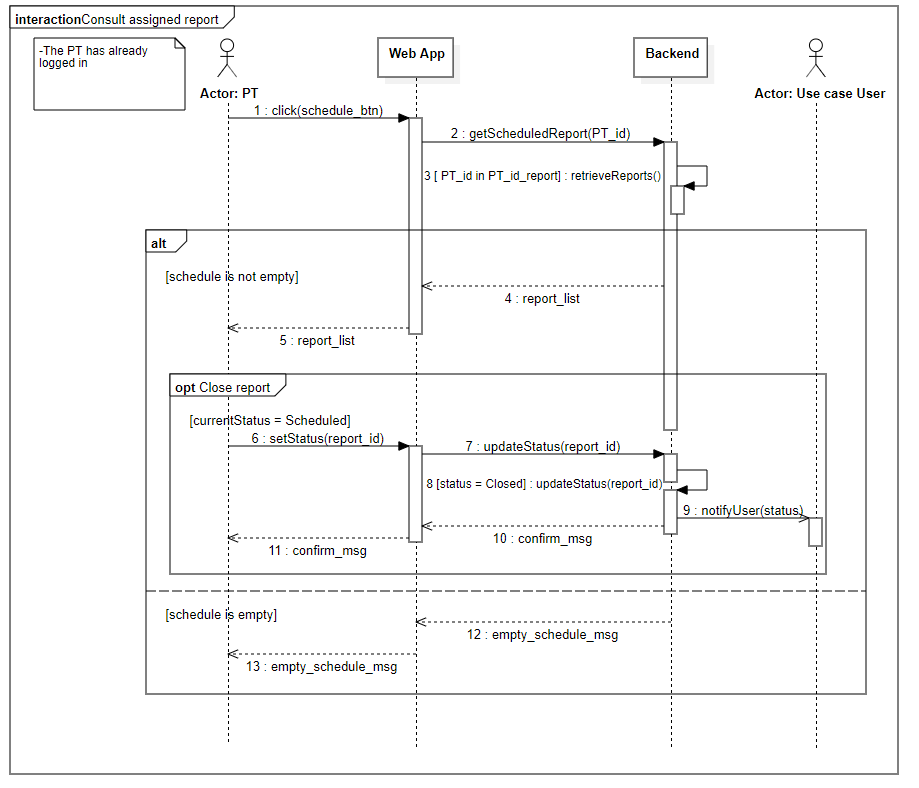
\includegraphics[width=\textwidth]{UML_diagrams/Sequence_Digrams/consult_assigned_report_sd.png}
  \caption{Consult assigned report sequence diagram}
  \label{fig:consult_assigned_report_sd}
\end{figure}

\begin{figure}[H]
  \centering
  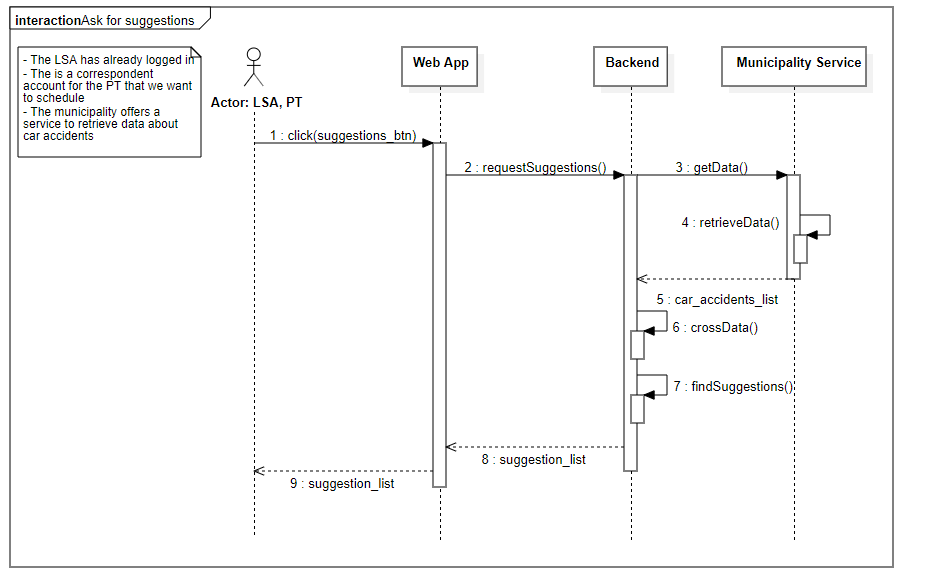
\includegraphics[width=\textwidth]{UML_diagrams/Sequence_Digrams/ask_suggestion_sd.png}
  \caption{Ask for suggestion sequence diagram}
  \label{fig:ask_suggestion_sd}
\end{figure}



\subsection{Use case diagrams}
\subsubsection{User}

\vfill

\begin{figure}[H]
  \centering
  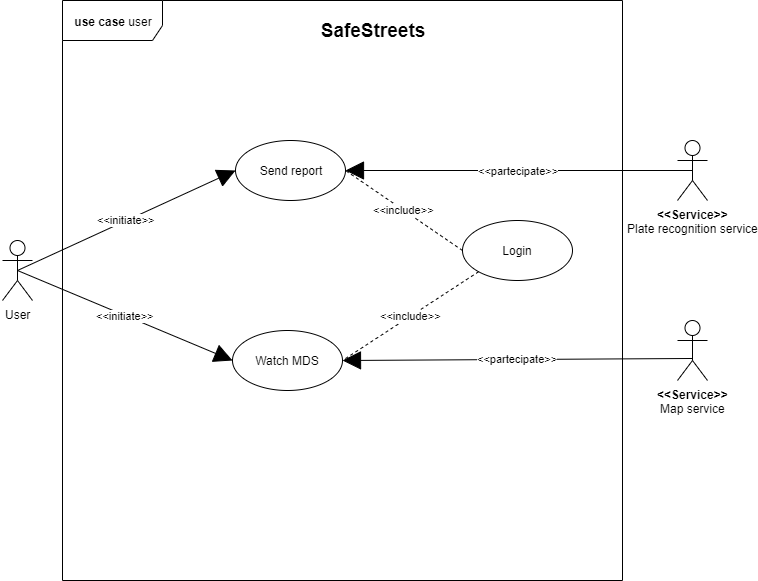
\includegraphics[width=\textwidth]{UML_diagrams/ucd_user.png}
  \caption{User use case diagram}
  \label{fig:user_ucd}
\end{figure}

\vfill
\newpage
\null


\subsubsection{Authorities}
In Fig \ref{fig:authority_ucd}, the Authority Login use case displayed in the following diagram is not related to any use case enlisted in section \ref{use_cases}. That is because the Login use case for the authority is basically the same as the user's one, indeed the only thing that changes is that the actor performs the login on the Web application instead of the mobile application.

\vfill


\begin{figure}[H]
  \centering
  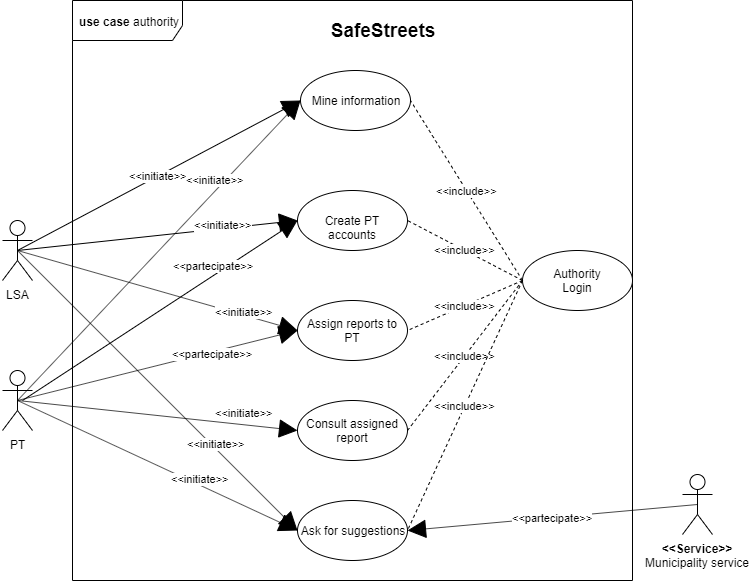
\includegraphics[width=\textwidth]{UML_diagrams/ucd_authority.png}
  \caption{Authority use case diagram}
  \label{fig:authority_ucd}
\end{figure}

\vfill
\newpage



  \section{Performance requirements}
  In order to promptly tackle violations that are reported,
SafeStreets has to be a low latency service: police technicians have
to intervene quickly, in order to fine the transgressors before they
leave the scene of the violation. Also, the system has to guarantee an
efficient service to an high number of users and police technician connected
simultaneously.
  \section{Design constraints}
  \subsection{Regulatory policies}
The user information is stored accordingly to the GDPR policies in order to guarantee the privacy of individuals.
\begin{itemize}
    \item No data is shared with third parties for commercial purposes;
    \item All reported images and violation data are stored safely through encryption methods. The third party system used for image recognition can not store any information/image which identifies;
    \item Any additional information, such as GPS position or Camera access, is promptly asked to the user before performing the specific operation, accordingly to the Android/IOS standards.
\end{itemize}


\subsection{Hardware limitations}
\begin{itemize}
    \item Mobile applications:
    \begin{itemize}
        \item Any kind of modern smartphone;
        \item Internet connectivity;
        \item Camera;
        \item GPS.
    \end{itemize}
    \item Web application:
    \begin{itemize}
        \item Browser (any HTTP client);
        \item Internet connectivity.
    \end{itemize}
\end{itemize}

\subsection{Interface to other applications}
\begin{itemize}
    \item A certified external image recognition service deals with the car plate recognition through report's images;
    \item Report's information are stored in a cloud database which guarantees data encryption and information retrieving through authentication;
    \item The municipality information center is periodically asked to provide data about the car accidents that happen among the municipality's territory.
\end{itemize}

  \section{Software system attributes}
  \subsection{Reliability}
The system needs to always be online in order to correctly store and 
manage violation reports and to be robust in case of failures. These 
requirements can be guaranteed through a virtual replication of the 
backend system: a possible solution
could be implemented through Docker containers managed by a container
orchestrion such as Kubernetes or DockerCompose. The container architecture
automatically restarts containers in case of failures (fault tollerant)
guaranteeing the system functioning in every situation.
\subsection{Availability}
As previously stated, the system must always guarantee an operating service of
violation reports. Thus, the system has to be available 
under stressing condition of an high number of users.
\subsection{Security}
As the data transferred and stored in the SafeStreets system deals with
private citizen's data, it must be guaranteed an high level of security.
In order to meet the GDPR conditions, all data has to be correctly 
encrypted through several security methods before being sent and stored.
\subsection{Maintainability}
The software maintainability is one of the most critical aspect in the
development of this software. In order to allow cheap and easy fix, SafeStreets
is developed by using several design patterns that make the software
flexible and scalable. Such patterns can be recognized both in the previous
UML class diagram and in further documents.
\subsection{Portability}
SafeStreets is intended to work on every mobile device, thus the technologies
used for its development have to be cross-platform (such as Flutter or any other
language which can generate applications for IOS and Android systems).

  \chapter{Formal analysis using Alloy}
  \section{Overview}
  In this	section an analysis of some critical aspects of the system is provided exploiting Alloy.	
The	focus is on	some static	constraints, in	particular:	
\begin{itemize}
    \item Uniqueness of usernames and every other univoque parameter of the system, such as plates, violationIds and so on;
    \item Users can only mine information concerning MDS and not Plates. Also they cannot explicitly query reports that has been performed by other users;
    \item LSAs can deal only with violation occurred in their competence area and thus scheduling such violations to the technician that they manage;
    \item SuggestedIntervention can be generated only if at least one violation occurred in the same location of the suggestion.
\end{itemize}
Other constraints are specified for keeping a steady structure of the alloy model, in order to avoid dangling entities and preserving foreign constraints.\newline
Four different worlds have been generated in order to verify the correctness of the constraints.

  \section{Alloy code}
  \lstinputlisting[language=alloy]{Alloy/safestreets_model.als}
  \section{Worlds}
  In order to prove the correctness of the alloy model, some different real situation has been created by usign the world predicates.
Here are the generated world replicas by predicates:
\begin{itemize}
    \item 
        \begin{figure}[H]
            \centering
            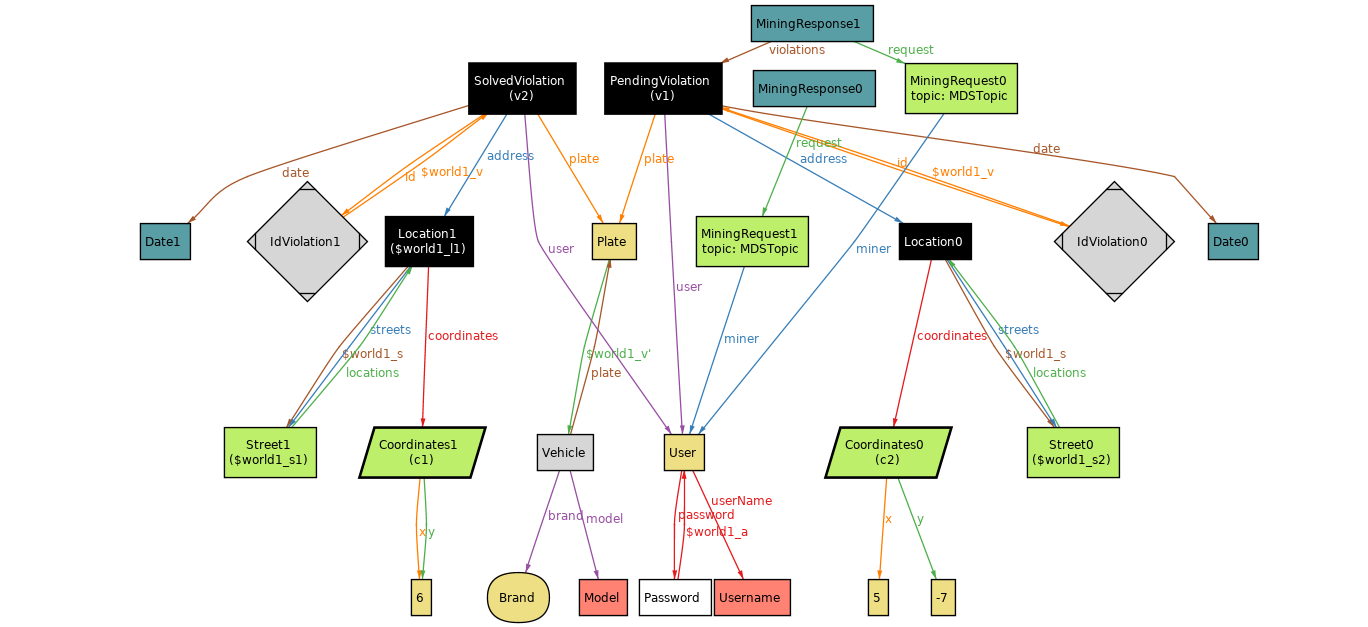
\includegraphics[width=1.0\textwidth]{alloy_world1}
            \caption{Alloy world 1}
            \label{fig:alloy_World1}
        \end{figure}
        \textit{World 1}: The first world pictures the situation in which a user publishes two different violation reports in different locations on different dates. Here is possible to underline the hierarchical relations between coordinates, locations and streets and the way reports are associated to users.
    \item 
        \begin{figure}[H]
            \centering
            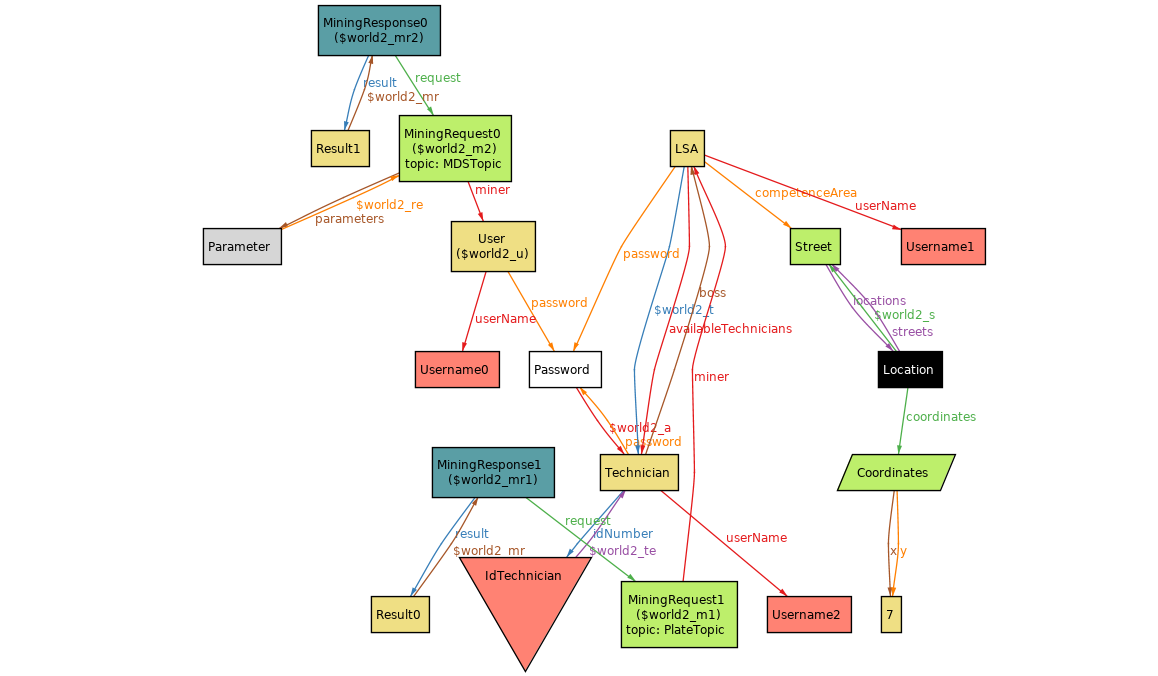
\includegraphics[width=1.0\textwidth]{alloy_world2}
            \caption{Alloy world 2}
            \label{fig:alloy_World2}
        \end{figure}
        \textit{World 2}: The second world pictures the situation in which different accounts have performed mining request on different topics. Here it is underlined that user can perform only MDS requests while technicians and LSAs can also be looking for Plate topics and deeper queries. Also, the number of parameters of each mining request have been limited to 3 for view purposes.
    \item 
        \begin{figure}[H]
            \centering
            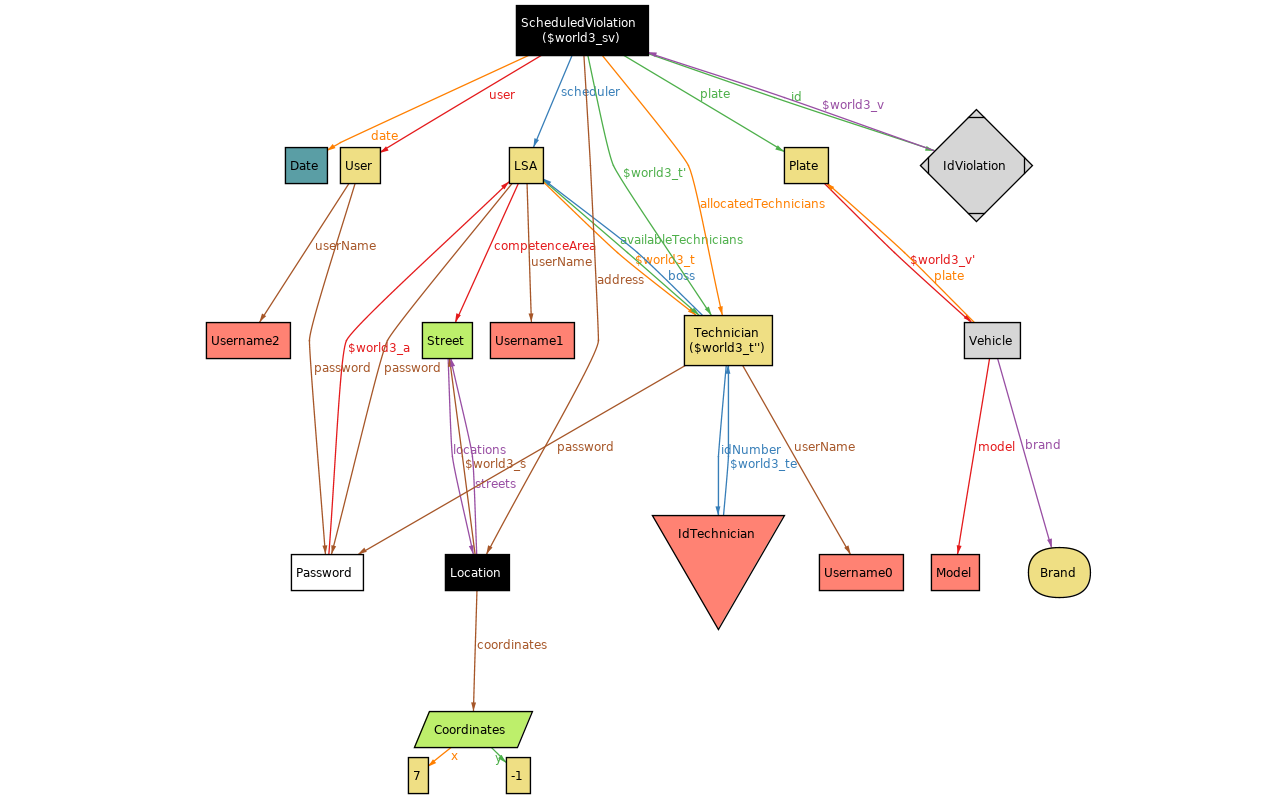
\includegraphics[width=1.0\textwidth]{alloy_world3}
            \caption{Alloy world 3}
            \label{fig:alloy_World3}
        \end{figure}
        \textit{World 3}: The third world pictures the situation in which a violation has been scheduled to a technician. Here the relations between technicians, scheduled violations and LSAs are underlined.
        \newpage
    \item 
        \begin{figure}[H]
            \centering
            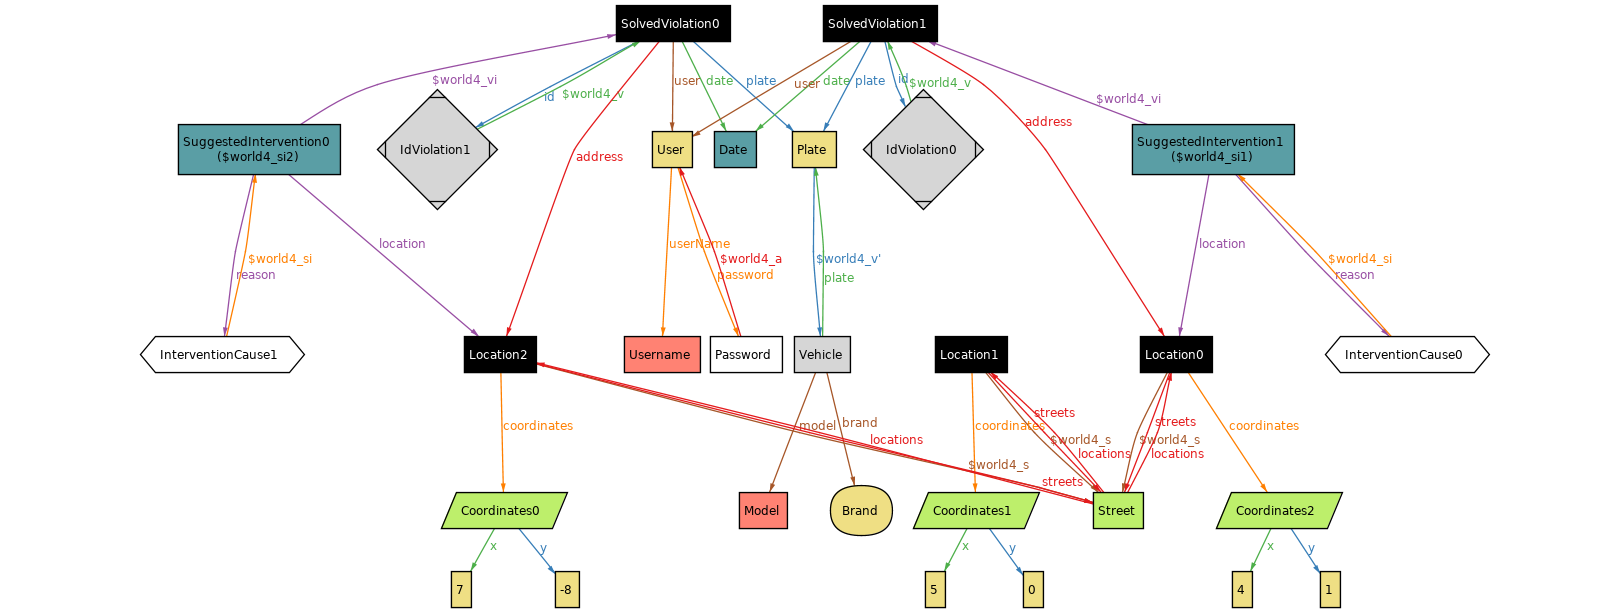
\includegraphics[width=1.0\textwidth]{alloy_world4}
            \caption{Alloy world 4}
            \label{fig:alloy_World4}
        \end{figure}
        \textit{World 4}: The fourth world pictures the situation in which a suggested intervention has been generated for a specific location. Here it is visible to have a look at the relations between suggested interventions, locations and violations. More specificly, it is possible to evince the fact that a suggested intervention can be performed on a certain location only if at least one violation occured at the same spot.
\end{itemize}
  \section{Alloy model performance}
  \begin{figure}[H]
    \centering
    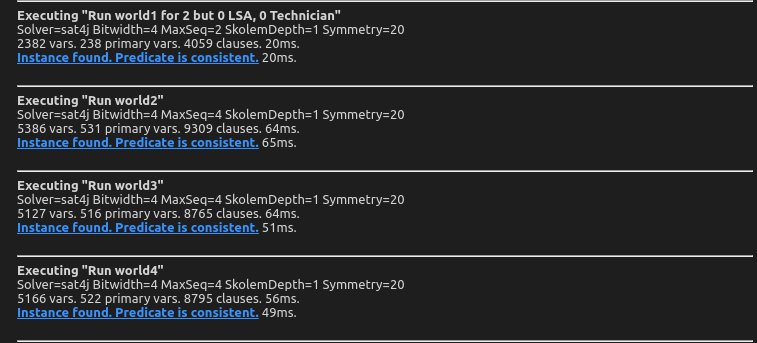
\includegraphics[width=1.0\textwidth]{alloy_performance}
    \caption{Alloy model performance}
    \label{fig:alloy_Performance}
\end{figure}

  \chapter{Effort Spent}
  \section{Luca Loria}
\begin{table}[H]
    \centering
    % \renewcommand{\arraystretch}{0.8}
    \begin{tabularx}{\textwidth}{ |l|c|X| }
        \hline
        Day & Hours & Topic \\
        \hline
        20/10/2019 & 1.5 & Text assumptions \\								
        \hline
        22/10/2019 & 1	& Domain assumptions \\
        \hline
        23/10/2019 & 2	& Design constraints \\
        \hline								
        24/10/2019 & 2	& Revision ch 1 and 2 \\									
        \hline
        26/10/2019 & 3 & Software system attributes \\									
        \hline
        28/10/2019 & 0.5 & Performance requirements \\									
        \hline
        29/10/2019 & 2	& External interface req \\									
        \hline
        30/10/2019 & 5 & Mockups creation \\									
        \hline
        31/10/2019 & 1.5 & Revision ch 3 \\									
        \hline
        01/11/2019 & 1 & Alloy signatures \\									
        \hline
        04/11/2019 & 1.5 & Alloy facts part 1 \\									
        \hline
        06/11/2019 & 3 & Alloy facts part 2 and world predicates \\						
        \hline
        07/11/2019 & 4 & Finish alloy, fix class diagram and start impaginating \\		
        \hline
        08/11/2019 & 3.5 & Reviewing requirements and sequence diagrams. Create references and Revision. Create alloy world section in RASD. Start impaginating correctly	\\
        \hline
        09/11/2019 & 2 & Shared phenomena matrix, frontpage and pagination fixes \\
        \hline							
    \end{tabularx}
  \end{table}

  \section{Nicolò Albergoni}
\begin{table}[H]
  \centering
  % \renewcommand{\arraystretch}{0.8}
  \begin{tabularx}{\textwidth}{ |l|c|X| }
      \hline
      Day & Hours & Topic \\
      \hline
      22/10/2019 & 2.5 & Purpose \\								
      \hline
      23/10/2019 & 3 & Scope, Current system \\
      \hline
      24/10/2019 & 1.75	& Goals, Overview\\
      \hline								
      26/10/2019 & 3	& Product perspective, Product function\\									
      \hline
      27/10/2019 & 3 & Product function, Revision ch 1 and 2 \\									
      \hline
      29/10/2019 & 2.5 & Scenarios \\									
      \hline
      30/10/2019 & 4 & Use cases \\									
      \hline
      31/10/2019 & 3 & Use cases, Revision ch 3 \\
      \hline
      01/11/2019 & 1 & Finish use cases \\									
      \hline
      02/11/2019 & 2.75 & Requirements \\									
      \hline
      05/11/2019 & 2.25 & Finish requirements \\									
      \hline
      06/11/2019 & 2.5 & Sequence diagrams \\									
      \hline
      07/11/2019 & 3.25 & Sequence diagrams \\						
      \hline
      08/11/2019 & 1.75 & Finish and reviewing of sequence diagrams \\
      \hline
      09/11/2019 & 2 & Use case diagrams, pagination fixes	\\
      \hline
      10/11/2019 & 2 & Traceability matrix, final revision	\\
      \hline        							
  \end{tabularx}
\end{table}


  \chapter{References}
  \begin{itemize}
    \item LateX Workshop extension for Visual Studio Code: \newline\href{https://github.com/James-Yu/LaTeX-Workshop/}{https://github.com/James-Yu/LaTeX-Workshop/}
    \item LateX compiler: \newline\href{https://www.latex-project.org/}{https://www.latex-project.org/}
    \item StarUML for UML diagrams:\newline\href{http://staruml.io/}{http://staruml.io/}
    \item DrawIO for some UML diagrams\newline\href{http://draw.io}{http://draw.io}
    \item MVC design pattern wikipedia: \newline\href{https://en.wikipedia.org/wiki/Model-view-controller}{https://en.wikipedia.org/wiki/Model-view-controller}
    \item Multitier architecture wikipedia: \newline\href{https://en.wikipedia.org/wiki/Multitier_architecture}{wikipedia}
    \item Relational database advantages: \newline\href{https://searchdatamanagement.techtarget.com/definition/relational-database}{https://searchdatamanagement.techtarget.com/definition/relational-database}
\end{itemize}
  \end{document}
  

  \loadspellchecklist[en][wordlist.txt]
  \setupspellchecking[state=start]